%!TEX TS-program = platex 

% Also note that the "draftcls" or "draftclsnofoot", not "draft", option
% should be used if it is desired that the figures are to be displayed in
% draft mode.
%
\documentclass[10pt, conference, compsocconf]{IEEEtran}
% Add the compsocconf option for Computer Society conferences.
%
% If IEEEtran.cls has not been installed into the LaTeX system files,
% manually specify the path to it like:
% \documentclass[conference]{../sty/IEEEtran}

\usepackage[dvipdfmx]{graphicx}


% *** MISC UTILITY PACKAGES ***
%\usepackage{ifpdf}
% Heiko Oberdiek's ifpdf.sty is very useful if you need conditional
% compilation based on whether the output is pdf or dvi.
% usage:
% \ifpdf
%   % pdf code
% \else
%   % dvi code
% \fi
% The latest version of ifpdf.sty can be obtained from:
% http://www.ctan.org/tex-archive/macros/latex/contrib/oberdiek/
% Also, note that IEEEtran.cls V1.7 and later provides a builtin
% \ifCLASSINFOpdf conditional that works the same way.
% When switching from latex to pdflatex and vice-versa, the compiler may
% have to be run twice to clear warning/error messages.

% *** CITATION PACKAGES ***
%
\usepackage{cite}
% cite.sty was written by Donald Arseneau
% V1.6 and later of IEEEtran pre-defines the format of the cite.sty package
% \cite{} output to follow that of IEEE. Loading the cite package will
% result in citation numbers being automatically sorted and properly
% "compressed/ranged". e.g., [1], [9], [2], [7], [5], [6] without using
% cite.sty will become [1], [2], [5]--[7], [9] using cite.sty. cite.sty's
% \cite will automatically add leading space, if needed. Use cite.sty's
% noadjust option (cite.sty V3.8 and later) if you want to turn this off.
% cite.sty is already installed on most LaTeX systems. Be sure and use
% version 4.0 (2003-05-27) and later if using hyperref.sty. cite.sty does
% not currently provide for hyperlinked citations.
% The latest version can be obtained at:
% http://www.ctan.org/tex-archive/macros/latex/contrib/cite/
% The documentation is contained in the cite.sty file itself.

% *** GRAPHICS RELATED PACKAGES ***
%
%\ifCLASSINFOpdf
  % \usepackage[pdftex]{graphicx}
  % declare the path(s) where your graphic files are
%  \graphicspath{{../pdf/}{../jpeg/}}
  % and their extensions so you won't have to specify these with
  % every instance of \includegraphics
%   \DeclareGraphicsExtensions{.pdf,.jpeg,.png}
%\else
  % or other class option (dvipsone, dvipdf, if not using dvips). graphicx
  % will default to the driver specified in the system graphics.cfg if no
  % driver is specified.
 %  \usepackage[dvips]{graphicx}
  % declare the path(s) where your graphic files are
  % \graphicspath{{../eps/}}
  % and their extensions so you won't have to specify these with
  % every instance of \includegraphics
  % \DeclareGraphicsExtensions{.eps}
%\fi
% graphicx was written by David Carlisle and Sebastian Rahtz. It is
% required if you want graphics, photos, etc. graphicx.sty is already
% installed on most LaTeX systems. The latest version and documentation can
% be obtained at: 
% http://www.ctan.org/tex-archive/macros/latex/required/graphics/
% Another good source of documentation is "Using Imported Graphics in
% LaTeX2e" by Keith Reckdahl which can be found as epslatex.ps or
% epslatex.pdf at: http://www.ctan.org/tex-archive/info/
%
% latex, and pdflatex in dvi mode, support graphics in encapsulated
% postscript (.eps) format. pdflatex in pdf mode supports graphics
% in .pdf, .jpeg, .png and .mps (metapost) formats. Users should ensure
% that all non-photo figures use a vector format (.eps, .pdf, .mps) and
% not a bitmapped formats (.jpeg, .png). IEEE frowns on bitmapped formats
% which can result in "jaggedy"/blurry rendering of lines and letters as
% well as large increases in file sizes.
%
% You can find documentation about the pdfTeX application at:
% http://www.tug.org/applications/pdftex





% *** MATH PACKAGES ***
%
%\usepackage[cmex10]{amsmath}
% A popular package from the American Mathematical Society that provides
% many useful and powerful commands for dealing with mathematics. If using
% it, be sure to load this package with the cmex10 option to ensure that
% only type 1 fonts will utilized at all point sizes. Without this option,
% it is possible that some math symbols, particularly those within
% footnotes, will be rendered in bitmap form which will result in a
% document that can not be IEEE Xplore compliant!
%
% Also, note that the amsmath package sets \interdisplaylinepenalty to 10000
% thus preventing page breaks from occurring within multiline equations. Use:
%\interdisplaylinepenalty=2500
% after loading amsmath to restore such page breaks as IEEEtran.cls normally
% does. amsmath.sty is already installed on most LaTeX systems. The latest
% version and documentation can be obtained at:
% http://www.ctan.org/tex-archive/macros/latex/required/amslatex/math/

% *** SPECIALIZED LIST PACKAGES ***
%
%\usepackage{algorithmic}
% algorithmic.sty was written by Peter Williams and Rogerio Brito.
% This package provides an algorithmic environment fo describing algorithms.
% You can use the algorithmic environment in-text or within a figure
% environment to provide for a floating algorithm. Do NOT use the algorithm
% floating environment provided by algorithm.sty (by the same authors) or
% algorithm2e.sty (by Christophe Fiorio) as IEEE does not use dedicated
% algorithm float types and packages that provide these will not provide
% correct IEEE style captions. The latest version and documentation of
% algorithmic.sty can be obtained at:
% http://www.ctan.org/tex-archive/macros/latex/contrib/algorithms/
% There is also a support site at:
% http://algorithms.berlios.de/index.html
% Also of interest may be the (relatively newer and more customizable)
% algorithmicx.sty package by Szasz Janos:
% http://www.ctan.org/tex-archive/macros/latex/contrib/algorithmicx/




% *** ALIGNMENT PACKAGES ***
%
%\usepackage{array}
% Frank Mittelbach's and David Carlisle's array.sty patches and improves
% the standard LaTeX2e array and tabular environments to provide better
% appearance and additional user controls. As the default LaTeX2e table
% generation code is lacking to the point of almost being broken with
% respect to the quality of the end results, all users are strongly
% advised to use an enhanced (at the very least that provided by array.sty)
% set of table tools. array.sty is already installed on most systems. The
% latest version and documentation can be obtained at:
% http://www.ctan.org/tex-archive/macros/latex/required/tools/


%\usepackage{mdwmath}
%\usepackage{mdwtab}
% Also highly recommended is Mark Wooding's extremely powerful MDW tools,
% especially mdwmath.sty and mdwtab.sty which are used to format equations
% and tables, respectively. The MDWtools set is already installed on most
% LaTeX systems. The lastest version and documentation is available at:
% http://www.ctan.org/tex-archive/macros/latex/contrib/mdwtools/


% IEEEtran contains the IEEEeqnarray family of commands that can be used to
% generate multiline equations as well as matrices, tables, etc., of high
% quality.


%\usepackage{eqparbox}
% Also of notable interest is Scott Pakin's eqparbox package for creating
% (automatically sized) equal width boxes - aka "natural width parboxes".
% Available at:
% http://www.ctan.org/tex-archive/macros/latex/contrib/eqparbox/





% *** SUBFIGURE PACKAGES ***
%\usepackage[tight,footnotesize]{subfigure}
% subfigure.sty was written by Steven Douglas Cochran. This package makes it
% easy to put subfigures in your figures. e.g., "Figure 1a and 1b". For IEEE
% work, it is a good idea to load it with the tight package option to reduce
% the amount of white space around the subfigures. subfigure.sty is already
% installed on most LaTeX systems. The latest version and documentation can
% be obtained at:
% http://www.ctan.org/tex-archive/obsolete/macros/latex/contrib/subfigure/
% subfigure.sty has been superceeded by subfig.sty.



%\usepackage[caption=false]{caption}
%\usepackage[font=footnotesize]{subfig}
% subfig.sty, also written by Steven Douglas Cochran, is the modern
% replacement for subfigure.sty. However, subfig.sty requires and
% automatically loads Axel Sommerfeldt's caption.sty which will override
% IEEEtran.cls handling of captions and this will result in nonIEEE style
% figure/table captions. To prevent this problem, be sure and preload
% caption.sty with its "caption=false" package option. This is will preserve
% IEEEtran.cls handing of captions. Version 1.3 (2005/06/28) and later 
% (recommended due to many improvements over 1.2) of subfig.sty supports
% the caption=false option directly:
%\usepackage[caption=false,font=footnotesize]{subfig}
%
% The latest version and documentation can be obtained at:
% http://www.ctan.org/tex-archive/macros/latex/contrib/subfig/
% The latest version and documentation of caption.sty can be obtained at:
% http://www.ctan.org/tex-archive/macros/latex/contrib/caption/




% *** FLOAT PACKAGES ***
%
%\usepackage{fixltx2e}
% fixltx2e, the successor to the earlier fix2col.sty, was written by
% Frank Mittelbach and David Carlisle. This package corrects a few problems
% in the LaTeX2e kernel, the most notable of which is that in current
% LaTeX2e releases, the ordering of single and double column floats is not
% guaranteed to be preserved. Thus, an unpatched LaTeX2e can allow a
% single column figure to be placed prior to an earlier double column
% figure. The latest version and documentation can be found at:
% http://www.ctan.org/tex-archive/macros/latex/base/



%\usepackage{stfloats}
% stfloats.sty was written by Sigitas Tolusis. This package gives LaTeX2e
% the ability to do double column floats at the bottom of the page as well
% as the top. (e.g., "\begin{figure*}[!b]" is not normally possible in
% LaTeX2e). It also provides a command:
%\fnbelowfloat
% to enable the placement of footnotes below bottom floats (the standard
% LaTeX2e kernel puts them above bottom floats). This is an invasive package
% which rewrites many portions of the LaTeX2e float routines. It may not work
% with other packages that modify the LaTeX2e float routines. The latest
% version and documentation can be obtained at:
% http://www.ctan.org/tex-archive/macros/latex/contrib/sttools/
% Documentation is contained in the stfloats.sty comments as well as in the
% presfull.pdf file. Do not use the stfloats baselinefloat ability as IEEE
% does not allow \baselineskip to stretch. Authors submitting work to the
% IEEE should note that IEEE rarely uses double column equations and
% that authors should try to avoid such use. Do not be tempted to use the
% cuted.sty or midfloat.sty packages (also by Sigitas Tolusis) as IEEE does
% not format its papers in such ways.

% *** PDF, URL AND HYPERLINK PACKAGES ***
%
%\usepackage{url}
% url.sty was written by Donald Arseneau. It provides better support for
% handling and breaking URLs. url.sty is already installed on most LaTeX
% systems. The latest version can be obtained at:
% http://www.ctan.org/tex-archive/macros/latex/contrib/misc/
% Read the url.sty source comments for usage information. Basically,
% \url{my_url_here}.


% *** Do not adjust lengths that control margins, column widths, etc. ***
% *** Do not use packages that alter fonts (such as pslatex).         ***
% There should be no need to do such things with IEEEtran.cls V1.6 and later.
% (Unless specifically asked to do so by the journal or conference you plan
% to submit to, of course. )


% correct bad hyphenation here
\hyphenation{op-tical net-works semi-conduc-tor}

% ************************
% 	Document start
% ************************


\begin{document}

\title{Toward Fine-grained GPU Resource Management using Microcontrollers}

% author names and affiliations
% use a multiple column layout for up to two different
% affiliations
\if 0
\author{\IEEEauthorblockN{Yusuke Fujii}
\IEEEauthorblockA{line 1 (of Affiliation): dept. name of organization\\
line 2: name of organization, acronyms acceptable\\
Shiga, Japan\\
yukke@ubi.cs.ritsumei.ac.jp}
\and
\IEEEauthorblockN{Takuya Azumi}
\IEEEauthorblockA{line 1 (of Affiliation): dept. name of organization\\
line 2: name of organization, acronyms acceptable\\
line 3: City, Country\\
line 4: Email: name@xyz.com}
\and
\IEEEauthorblockN{Nobuhiko Nishio}
\IEEEauthorblockA{line 1 (of Affiliation): dept. name of organization\\
line 2: name of organization, acronyms acceptable\\
line 3: City, Country\\
line 4: Email: name@xyz.com}
\and
\IEEEauthorblockN{Shinpei Kato}
\IEEEauthorblockA{line 1 (of Affiliation): dept. name of organization\\
line 2: name of organization, acronyms acceptable\\
line 3: City, Country\\
line 4: Email: name@xyz.com}
}
\fi

% conference papers do not typically use \thanks and this command
% is locked out in conference mode. If really needed, such as for
% the acknowledgment of grants, issue a \IEEEoverridecommandlockouts
% after \documentclass

% for over three affiliations, or if they all won't fit within the width
% of the page, use this alternative format:
% 
%\author{\IEEEauthorblockN{Yusuke Fujii\IEEEauthorrefmark{1},
%Takuya Azumi\IEEEauthorrefmark{1},
%Nobuhiko Nishio\IEEEauthorrefmark{1} and
%Shinpei Kato\IEEEauthorrefmark{2}}
%
%\IEEEauthorblockA{\IEEEauthorrefmark{1}Ritsumeikan University}
%\IEEEauthorblockA{\IEEEauthorrefmark{2}Nagoya University}
%}
\author{\IEEEauthorblockN{Yusuke Fujii, Takuya Azumi, and Nobuhiko
Nishio}
\IEEEauthorblockA{Department of Computer Science\\Ritsumeikan University}
\and
\IEEEauthorblockN{Shinpei Kato}
\IEEEauthorblockA{Department of Information Engineering\\Nagoya University}
}

% use for special paper notices
%\IEEEspecialpapernotice{(Invited Paper)}

% make the title area
\maketitle

\begin{abstract}
 Recent graphics processing units (GPUs) integrate wimpy
 microcontrollers on a chip.
 These microcontrollers are highly available to extend the functionality
 of GPU resource management, launching firmware code to control GPU
 executions and data transfers without accessing the host CPUs at all.
 In this paper, we develop a compiler and debugging environment for
 NVIDIA's GPU microcontrollers in order to enhance the productivity of
 GPU firmware development.
 Our compiler is implemented using the well-known portable LLVM compiler
 infrastructure, while together providing a debugging subsystem that can
 individually execute firmware on the microcontroller.
 As a proof of concept, we develop fully-functional firmware using our
 compiler and debugging environment, and evaluate it using an NVIDIA's
 graphics card. 
 Experimental results demonstrate that the overhead of introducing our
 firmware is suppressed to within 2.3\%, as compared to the native
 proprietary firmware.
 It is also identified that the impact of overhead is no greater than
 0.01\% of the total execution time of microbenchmark programs.
\end{abstract}

\begin{IEEEkeywords}
GPGPU; LLVM; Microcontrollers

\end{IEEEkeywords}




% For peer review papers, you can put extra information on the cover
% page as needed:
% \ifCLASSOPTIONpeerreview
% \begin{center} \bfseries EDICS Category: 3-BBND \end{center}
% \fi
%
% For peerreview papers, this IEEEtran command inserts a page break and
% creates the second title. It will be ignored for other modes.
\IEEEpeerreviewmaketitle


% Chapter1
%!TEX root = farm.tex

\section{Introduction}\label{sec:intro}
% no \IEEEPARstart

Graphics processing units (GPUs) are becoming more and more commonplace
to support compute-intensive and data-parallel computing.
In many application domains, GPU-accelerated systems provide significant
performance gains over traditional multi-core CPU-based systems.
As shown in Table~\ref{tab:cpu-gpu}, the peak performance of the
state-of-the-art GPUs exceeds 3,000 GFLOPS, integrating more than 1,500
cores on a chip, which is nearly equivalent of 19 times that of
traditional microprocessors, such as Intel Core i7 series.
Such a rapid growth of GPUs is due to recent advances in programming
support, such as CUDA\cite{cuda} and OpenCL\cite{opencl},  for
general-purpose computing on GPUs, also known as GPGPU.

\begin{table*}[tb]
 \caption{Comparison of the Intel CPU Architectures and the NVIDIA GPU
 Architectures}
 \label{tab:cpu-gpu}
 \begin{center}
  \hbox to\hsize{\hfil
  \begin{tabular}{|c|c|c|c|c|c|}\hline
   & Core i7 980XE & Core i7 3960X & GeForce GTX285 & GeForce GTX480 &
   GeForce GTX680 \\ \hline
   \# of processing cores & 6 & 6 & 240 & 480 & 1536 \\ \hline
   Single-precision performance (GFLOPS) & 108.0 & 158.4 & 933.0 & 1350.0
		   & 3090.0 \\ \hline
   Memory bandwidth (GB/sec) & 37.55 & 51.2 & 159.0 & 177.0 & 192.2 \\ \hline
   Power consumption (watt) & 130 & 278 & 183 & 250 & 195 \\ \hline
   Release date & 2010/03 & 2011/11 & 2009/01 & 2010/04 & 2012/03 \\ \hline
  \end{tabular}\hfil}
 \end{center}
\end{table*}

\par
In recent years, real-time systems have been augmented with
the GPU~\cite{Kato_ATC11, Kato_RTSS11, Kato_RTAS11, Basaran_ECRTS12,
Elliott_ECRTS12, Elliott_RTS12}.
The motivation of using the GPU in real-time systems is mainly found in
emerging applications of cyber-physical systems~\cite{Aumiller_CPSNA12,
McNaughton_ICRA11, Ferreira_JRTIP11}, where a large
amount of data acquired from the physical world needs to be processed in
real-time.
Given that the workload of such applications is highly compute-intensive and
data-parallel, many-core computing on the GPU is best suited to meet the
real-fast requirements of computation.
What is challenging in this line of work is to control the GPU under
real-time constraints.
The GPU is a coprocessor independent of the CPU, and hence two different
pieces of code are running concurrently on the GPU and the CPU, respectively.
This heterogeneity poses a core challenge in resource management.
Since the GPU is designed to accelerate particular workload, resource
management functions are often performed on the CPU.
In other words, the GPU and the CPU must be synchronized in some way to
ensure timeliness.
Unfortunately, this could be a major source of latency that makes
real-time systems unpredictable~\cite{Kato_ATC11}, though the previous
work are forced to take this approach due to a lack of functionality
that enables resource management functions to offload on to the GPU.
While compute cores or shaders on the GPU are not available to perform
resource management, recent GPUs integrate microcontrollers on a chip
where firmware code is launched to control the functional units of the
GPU.
These microcontrollers are highly available to extend the functionality
of GPU resource management, launching special pieces of firmware code to
control GPU executions and data transfers.

\par
This paper presents a compiler and debugging environment for NVIDIA's
GPU microcontrollers based on the well-known portable LLVM compiler
infrastructure.
The main purpose of this environment is to enhance the productivity of
GPU firmware development so that the community can facilitate future
research on fine-grained GPU resource management using microcontrollers.
Firmware is self-contained within the GPU, and there will be
interference from background jobs running on the CPU, once it is
uploaded by the device driver.
Therefore, we believe that GPU computing would be more timely and
reliable for real-time systems, if the firmware can support GPU resource
management by itself.
In this paper, we develop an initial stage of the firmware, and evaluate
its basic performance.

\par
The rest of this paper is organized as follows.
Section~\ref{sec:intro} introduces the underlying platform technology.
Section~\ref{sec:tech} describes the design and implementation of our
compiler and debugging environment for NVIDIA's GPU microcontrollers,
and Section~\ref{sec:evaluation} evaluates its basic performance.
Related work are discussed in Section~\ref{sec:related}.
This paper is concluded in Section~\ref{sec:con}.
\stepcounter{footnote}

% Chapter2
%!TEX root = farm.tex

\section{Platform Technology}\label{sec:tech}

First of all, we describe the platform technology underlying our
development.
We intensively focus on NVIDIA's GPU architectures, while the idea of
integrating GPU resource management into on-chip microcontrollers is not
limited to these specific architectures.
All pieces of technology presented herein are open-source, and may be
downloaded from the corresponding websites, respectively.

\subsection{Assembler for GPU microcontrollers}\label{sec:envy}

The assembler is comprised in package of the Envytools suite~\cite{envytools}.
The Envytools suite is a rich set of open-source tools to compile or
decompile GPU shader code, firmware code, macro code, and so on. 
It is also used to generate header files of GPU command definitions used
by the device driver and the runtime library.
There are many other useful tools and documentations for NVIDIA's GPU
architectures enclosed in the Envytools suite.

\subsection{GPU Device Driver}\label{sec:driver}

In general, the application programming interface (API) for the GPU is
provided by the runtime library.
GPU resource management, on the other hand, is often supported by the
device driver and the operating system (OS) module~\cite{Kato_ATC11,
Kato_ATC12, Bautin_MCNC08}.
As part of resource management, the device driver communicates with
microcontrollers integrated on the GPU.
The communication is typically managed by specific commands, which can
be handled by firmware running on each microcontroller.

\par
The firmware is built into the device driver by a shape of byte code,
and is uploaded on to the GPU at boot time.
To do so, we require open-source software, because we have to build the
firmware into the device driver.
In this paper, we use Gdev~\cite{Kato_ATC12}, an open-source module of
the GPGPU device driver and runtime library.

\subsection{LLVM Infrastructure}

The LLVM (Low Level Virtual Machine) project is a collection of
open-source modular and reusable compiler tool sets.
Since the microcontroller has its own instruction set architecture, we
develop an architecture-dependent backend of LLVM so that we can make
use of all the front-end modules of LLVM.

Figure \ref{fig:llvm} illustrates the structure of LLVM.
It first generates the LLVM IR (Intermediate Representation) from the
source code. 
This IR code is assembled by the LLVM backend.
The assembly code is finally translated to the object code for the
target machine.

\begin{figure}
\begin{center}
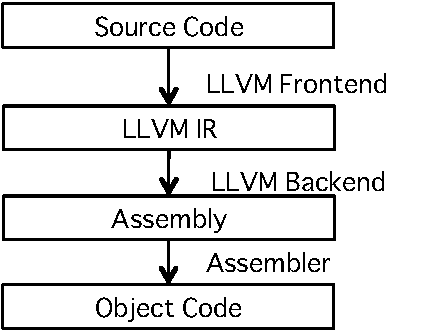
\includegraphics[scale = 0.5]{./img/llvmflow.pdf}
\end{center}
\caption{Compilation stages of LLVM.}
\label{fig:llvm}
\end{figure}

\subsubsection{LLVM IR}

The LLVM IR is an intermediate language used in LLVM, also called bitcode or
LLVM assembly languages.
This intermediate language is very powerful, scalable, light-weight, and
low-level enough to underlie many languages on top of many
architectures.
LLVM uses an expression of SSA (Static Single Assignment), which is
suitable for a lot of compiler optimization algorithms.

\subsubsection{LLVM frontend}\label{set:clang}

The LLVM frontend generates an intermediate language from a high-level
language in LLVM.
It is mainly used for code generation and its optimization.
In particular, we use Clang for our development, which is an open-source
compiler for the C family of programming languages provided by LLVM.

\subsubsection{LLVM backend}\label{set:backend}

The LLVM backend generates target code from an intermediate language in
LLVM.
The backend of LLVM features a target-independent code generator that
may create output for several types of target processors including X86,
PowerPC, ARM, and SPARC. 
This backend framework may also be used to generate code targeted at
accelerators such as Cell B/E and GPUs.
In fact, NVIDIA has announced recently that they use LLVM for the basis
of their CUDA compiler.
The backend of LLVM is composed of the LLC (LLVM static Compiler) and
the LLI (LLVM Interpreter).
LLI is an interpreter of the LLVM IR, also available as a JIT compiler,
while LLC is a static compiler to generate code.
We use this backend part of LLVM to generate code targeted at NVIDIA's
GPU microcontrollers.


% Chapter3
%!TEX root = farm.tex

\section{Compiler and Debugging Environment}\label{sec:design}

This section describes the design and implementation of our compiler and
debugging environment for NVIDIA's GPU microcontrollers.

\subsection{Microcontroller}

\begin{table}[tb]
\caption{Specification of GF100 microcontroller.} 
\label{tab:fermi}
\hbox to\hsize{\hfil
\begin{tabular}{|l|r|r|}\hline
Name 		&	HUB	   & GPC\\\hline
Architecture &	Fermi   & Fermi \\\hline
Number of units	& 1 & 4\\\hline
Bit 		&	32bit  & 32bit\\\hline
Code size  &	16,384 byte  & 8,192 byte\\\hline
Data size  &	4,096 byte  & 2,048 byte\\\hline
% \multicolumn{4}{l}{type-1\,: enumerate$BEy(B\quad type-2\,: enumerate*$BEy(B}\\
% \multicolumn{4}{l}{type-3\,: Enumerate$BEy(B\quad type-4\,: ENUMERATE$BEy(B}\\
\end{tabular}\hfil}
\end{table}

This paper presumes the microcontroller of NVIDIA's Fermi architecture.
In particular, we target the GeForce GTX 480 graphics card designed
based on the GF100 architecture.
In this architecture, a streaming multiprocessor (SM) consists of
32 CUDA cores, while a graphics processing cluster (GPC) consists of 4
SM's.
There are four GPC's in total equipped in the GF100 architecture, and
hence the maximum number of CUDA cores is 512.

Table~\ref{tab:fermi} illustrates the specification of the GF100
microcontroller.
There are two types of microcontrollers, HUB and GPC, relevant to CUDA
engines.
HUB is broadcasting the access to all GPC's, while the GPC represents a
specific microcontroller for each GPC engine.
Since the maximum code size is limited to 16KB as indicated in Table
\ref{tab:fermi}, developers should carefully design the firmware.

\subsection{Compiler Implementation}

\begin{figure*}
\begin{center}
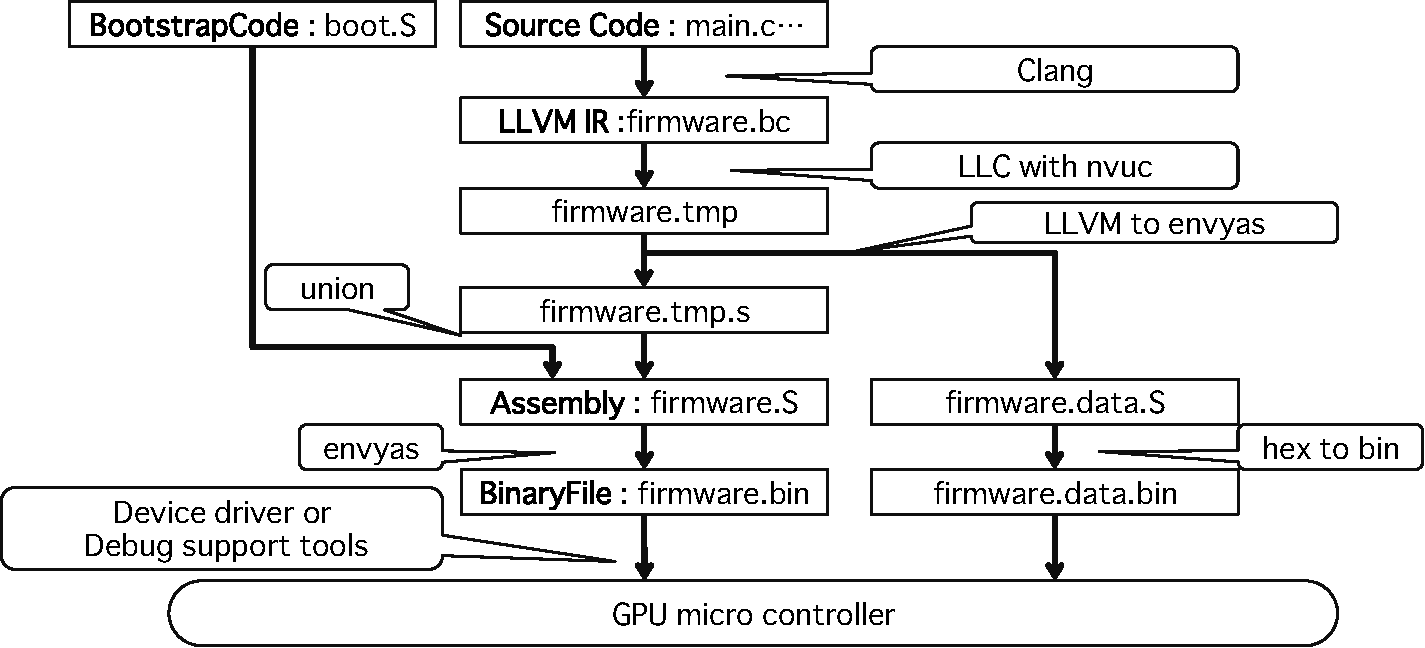
\includegraphics[width=12cm]{./img/step_compiler.pdf}
\end{center}
\caption{Overview of Compiler Implementation.}
\label{fig:compiler}
\end{figure*}

Figure \ref{fig:compiler} shows an overview of our compiler
implementation.
The main flow of compilation is done by Clang.
It generates the LLVM IR from the C source file.
The LLC next generates assembly code, which contains code and data in
separate files.
Finally, the Envytools outputs an executable file.
This executable file can be launched by the device driver, and can also
be tested by our debugging tool described in the later section.
To summarize, our compiler takes the following stages:

\begin{figure}
 \begin{center}
  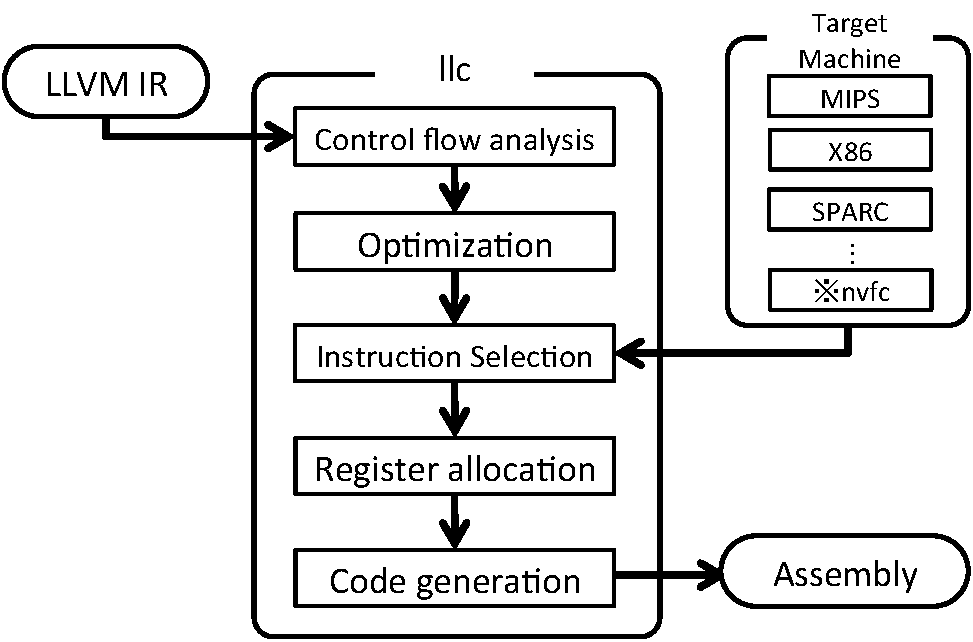
\includegraphics[width=6cm]{./img/llc.pdf}
 \end{center}
 \caption{Code generation stages of LLC.}
 \label{fig:llc}
\end{figure}

\begin{figure*}
 \begin{center}
  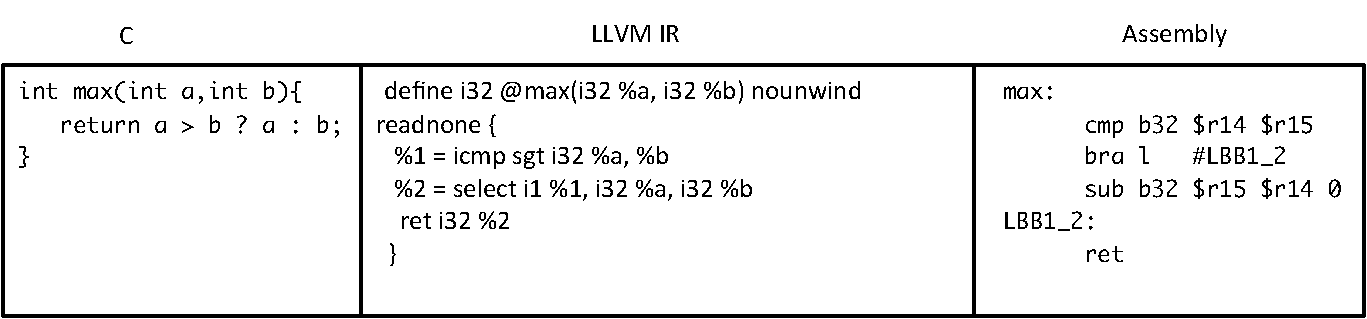
\includegraphics[width=12cm]{./img/llvm_code.pdf}
 \end{center}
 \caption{Examples of C source code and output code.}
 \label{fig:llvm_code}
\end{figure*}

\begin{description}
\item[ (1) Clang]\mbox{}\\
	   This is a frontend of C language that generates LLVM IR code
	   from the source file.

\item[ (2) LLC with nvuc]\mbox{}\\
	   This is a backend of LLVM that compiles LLVM IR code into
	   assembly code. 
	   As shown in Figure~\ref{fig:llc}, there are five steps to
	   exploit compilation: (i) flow analysis, (ii) optimization,
	   (iii) instruction selection, (iv) register allocation, and
	   (v) code generation.
	   This flow is not dependent on the target machine.
	   The LLC reads a configuration of the target machine at the
	   time of instruction selection, and selects a set of the
	   instruction and register to meet the specifications of each
	   machine.
	   Our implementation adds a new configuration called nvuc
	   (NVIDIA Micro-Controller) to support NVIDIA's GPU
	   microcontrollers under the LLVM infrastructure.

\item[ (3) LLVM to envyas]\mbox{}\\
	   This stage divides the generated assembly code into code and
	   data sections so that we can create binary images using
	   ``envyas'', which is a microcontroller assembler provided by
	   the Envytools suite.
	   The bootstrap code is also unified into the binary images
	   in this stage.
\item[ (4) envyas]\mbox{}\\
	   This is a final assembly stage for the microcontroller, which
	   generates the byte code of the firmware.
\item[ (5) hex to bin]\mbox{}\\
``hex to bin'' converts to the data portion split Step (3) to an executable file.

\item[ (6) Running the firmware]\mbox{}\\
There are two ways to run the firmware: incorporating the firmware into the device driver, or using the debugging support tool.
The device driver and the debugging support tool load the binary file of the firmware at boot time.
\end{description}

Figure \ref{fig:llvm_code} shows example of C language source codes, LLVM IR code, and assembly code.
Left is C language source codes, center is LLVM IR code that is generated by \ref{section:flow}(1), right is assembly code that is generated by \ref{section:flow}(3).

\begin{figure}
\begin{center}
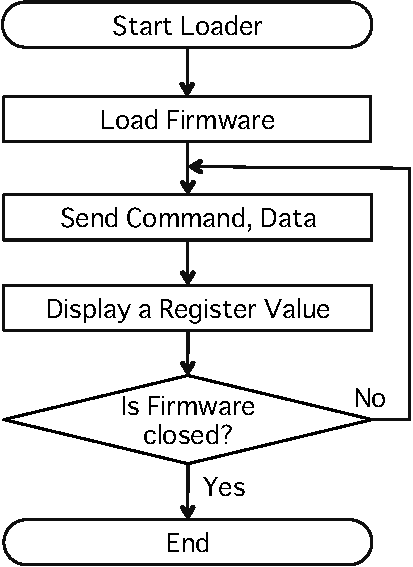
\includegraphics[width=3cm]{./img/loader.pdf}
\end{center}
\caption{Flowchart of Debugging Support Tool}
\label{fig:loader}
\end{figure}

\begin{figure*}
\begin{center}
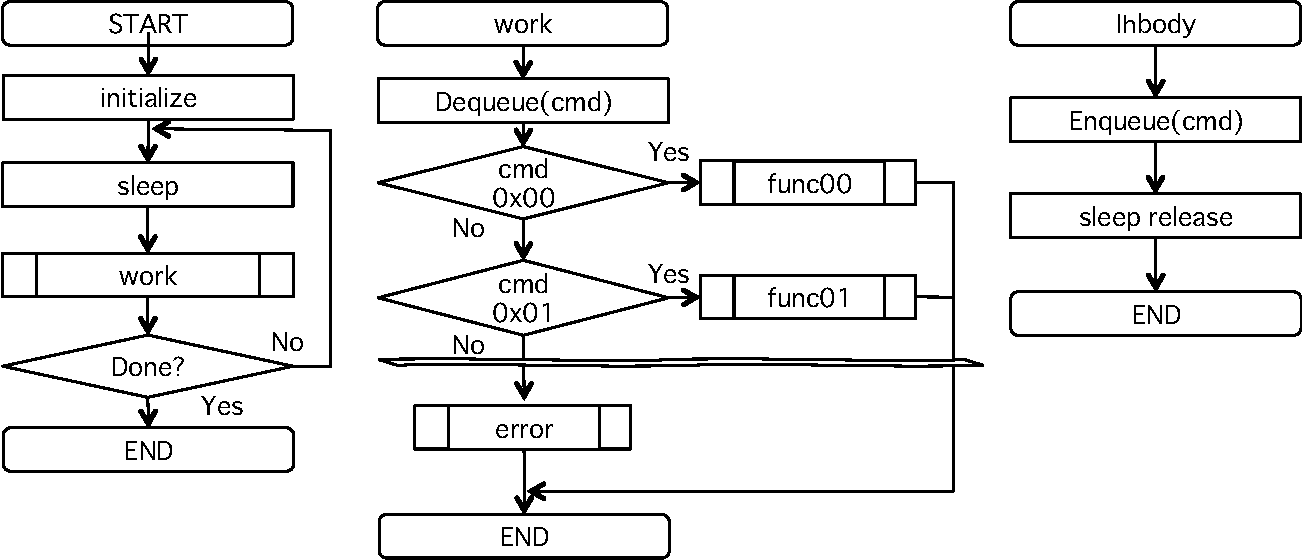
\includegraphics[width=12cm]{./img/firmware.pdf}
\end{center}
\caption{Flowchart of Our Firmware }
\label{fig:firmware}
\end{figure*}


\subsection{Debugging support tool}
Debugging support tool is to load the firmware, to send commands and data, and to display a register value of GPU.
Figure \ref{fig:loader} shows the flow of this tool flow, we describe use it.
Microcontrollers memory space map to  CPU memory space in MMIO (Memory Mapped IO).

\begin{description}
\item[ (1) Load the firmware]\mbox{}\\
Debugging support tool load the HUB firmware and GPC firmware executable code to mapping address by MMIO. 
After the load completion, this firmware runs by set a flag in the specified register.
\item[ (2) Sends commands and data]\mbox{}\\
A processing on microcontroller is suspended until receives a command.
The debugging support tool sends the command.
After an interrupt is executed by the command, the processing is resumed,

\item[ (3) Display a register] \mbox{}\\
The microcontroller has the register may be used freely on the host side.
The register is used for execute completion flag by the traditional firmware.
Thus we assumed that the register is used for the same purpose during debugging time, 
the register value is displayed.
\end{description}


\subsection{Firmware development}
In this section, we describe the our developing firmware on HUB.
Figure \ref{fig:firmware} shows that firmware flow chart.
The Firmware is started by setting the value in the register.

\begin{description}
\item[ (1) initialize]\mbox{}\\
The firmware sets the interrupt handler and get the data when started.
Next then Step(2).
\item[ (2) sleep]\mbox{}\\
The firmware makes the shift to the standby state, which wait for the receive command by the device driver or the debug support tools.
The firmware interrupt occurs when the firmware received command, which started ``ihbody''. 

\item[ (3) ihbody] \mbox{}\\
``ihbody'' enqueued command, and then it releases wait state of firmware.
\item[ (4) work] \mbox{}\\
``work'' function is called when the wait state of firmware is released.
``work'' calls the function after the dequeue.
It will check the end flag of firmware after the function execution.
\end{description}
We can recognize from what has been said that the firmware controlled by execute the function is better suited command.


% Chapter4
%!TEX root = farm.tex


\section{Evaluation}\label{sec:evaluation}
The evaluation compare the performance of the NVIDIA's standard firmware and we developed firmware used FARM.
Table \ref{tab:environment} shows the evaluation environment.
This evaluation measure the overhead of measuring the execution time in the NVIDIA's firmware and the we developed firmware on Gdev\cite{kato:gdev}\cite{kato:gdev2} of GPGPU runtime and resource management engine set.
This execution time is the time to copy of the data into device, the process execution, 
the copy of the data into host.
\par
Measurement results were concentrated in the following over 7msec and less 2msec.
This phenomenon occurred both firmware.
That because GPU's program are many things influence compared to the CPU Program.
Specifically, these are device memory, device driver, GPU cache and GPU memory.
Thus we divide over 7 msec are ``case A'', and less 2 msec are ``case B''.
We compare the average each case A and case B.
Figure \ref{fig:goodcase} shows result of case A.
Also figure \ref{fig:badcase} shows result of case B.
The abscissa axis is Sample program name.
The vertical axis is Execution time (msec).
The blue is the NVIDIA's standard firmware, also the red is the we developed firmware.
Figure \ref{fig:goodcase}, \ref{fig:badcase} can be as seen almost no overheads. 
It is the largest overhead, the case A is 0.003msec of madd, it was 2.31\%.
also it was the lowest overhead, the case B is -0,002msec, it was -1.74\%.
In this way, result has been increased execution time and decreased execution time.
Thus, it is within the range of error at execution time from a range of numbers that was measured is wide.
In addition, if you want to use the GPU application, there will be less affected because the processor core for processing time increases.
For example, The total time of madd in NVIDIA'S standard firmware is 21.842msec, this total time is between finished program from the start program by host.
The execution time overhead occupy relatively small 0.01\% of the total time
Thus, the overhead of firmware developed by our development environment is within the allowable range.
It follows from what has been said that developing firmware by this our development environment is a valid one.
\par
The total time includes the time required to generate GPU context, Memory allocation and Memory release time. 
madd by the running NVIDIA's standard firmware
The total time is 214 msec at the madd first execution times by the NVIDIA standard firmware.
The second total time is 20 msec, this result is a big gap to the first execution time.
Further, the our developing firmware get the same results to NVIDIA standard firmware.
Because the firmware generate the GPU context when the first run, and then, the firmware secondly running use GPU context generated by the first run.
Thus, it takes a long time to generate the GPU context.
This problem findings obtained by firmware development and evaluate.

\begin{table}[!t]
 \caption{Evaluate Environment} 
 \label{tab:environment}
 \hbox to\hsize{\hfil
 \begin{tabular}{|l|l|}\hline
  CPU &  Intel core i7 2600 \\\hline
  GPU &  NVIDIA GeForce GTX480 \\\hline
  Memory & 8GB \\\hline
  Kernel & Linux 2.6.42.12-1.fc15.x86\_64 \\\hline
  Device driver & PSCNV \\\hline
 \end{tabular}\hfil}
\end{table}

\begin{figure}
\begin{center}
\hfil
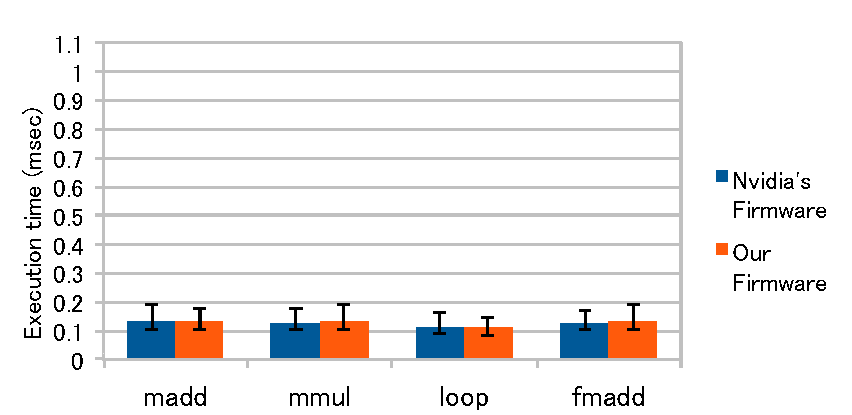
\includegraphics[width=8cm]{./img/good_case.pdf}
\end{center}
\caption{Execution Time of Gdev Sample Program : Case A}
\label{fig:goodcase}
\end{figure}

\begin{figure}
\begin{center}
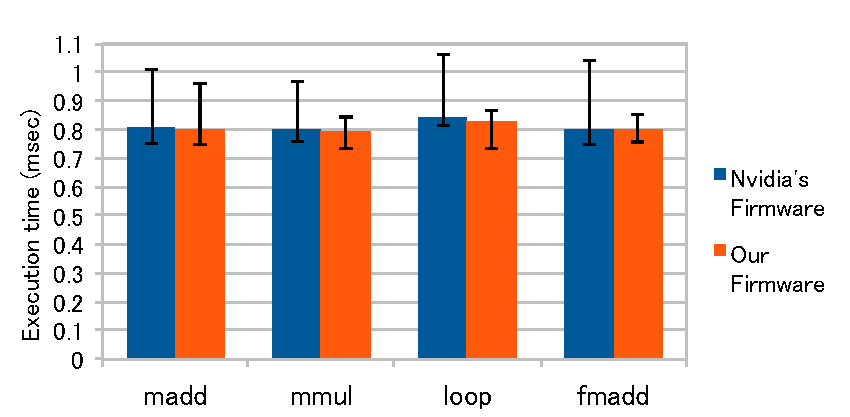
\includegraphics[width=8cm]{./img/bad_case.pdf}
\end{center}
\caption{Execution Time of Gdev Sample Program : Case B}
\label{fig:badcase}
\end{figure}



% Chapter5
%!TEX root = farm.tex

\section{Related Work}\label{sec:related}

We now briefly discuss related work, and draw a comparison with our
research. 

Helios~\cite{NightingaleEB:SOSP09:2009} is an operating system component
designed to simplify the task of writing, deploying, and tuning
applications for heterogeneous platforms.
They insist that programmable devices such as GPUs and NICs for the high-performance vector processing and high-speed communications.
GPU and NIC leveraging its capabilities via the device driver, in this form, the amount of data that can be transferred is limited by the communication between the CPU and the device.
Further more, the problem has complexity of the device driver and not provided interface of runs a task.
Approach is providing OS called Helios.
The Helios has micro kernel called satellite kernels.
The satellite kernels has the scheduler, memory manager, name space manager, and communication between the kernel.
The same direction that the Helios is our aim.
Helios approach to NIC, but our approach to GPU.
The above problems be able to solve by the  implement firmware on GPU microcontroller.

\subsection{Design of Direct Communication Facility for Manycore based Accelerators}
A study on DCFA\cite{weko_81351_1} was made by Si at the Tokyo university, and it revealed that the DCFA avoid the trouble of having to the communication latency of between devices by direct communication between devices without going through the host.
Currently, the DCFA can not adapt to the GPU, because the device address isn't known GPU.
We think that communication is done between the GPU devices by issuing to direct communication by the firmware.


% Chapter6
%!TEX root = farm.tex

\section{Conclusion}\label{sec:con}

In this paper, we have presented a new compiler and debugging
environment for NVIDIA's GPU microcontrollers.
As a basis of future work toward fined-grained GPU resource management,
we developed new firmware for those microcontrollers using our
development environment.
We executed several microbenchmark programs to demonstrate that the
overhead introduced by our firmware was no greater than 2.31\% of the
total execution, as compared to NVIDIA's proprietary firmware blob,
while our firmware even outperformed NVIDIA's firmware depending on test
cases.
One of the interesting findings obtained through the experiments was the
overhead of generating the GPU context, which must be minimized and
bounded in real-time systems.
Our development environment is all open-source, and may be download from
our web site~\cite{GIT_GDEV, GIT_FARM, GIT_NVFC}.

In future work, we pursue a new direction of GPU resource management
using microcontrollers.
First of all, the CPU load could be reduced by offloading GPU resource
management functions on to the GPU microcontroller.
This idea in fact is inspired by the Helios
project~\cite{Nightingale_SOSP09}, where networking resource management
functions are offloaded onto the NIC microcontroller.
Preemption support and power management for the GPU could also be
achieved by extending the firmware, as discussed in \cite{Kato_OSPERT11}.
We believe that such a fine-grained GPU resource management approach is
significant for real-time systems augmented with the GPU.


\bibliography{refer}
\bibliographystyle{IEEEtran}


% that's all folks
\end{document}


